\documentclass[12pt,english]{rftthesis}

\usepackage[utf8]{inputenc}
\usepackage[T1]{fontenc}
\usepackage[nottoc]{tocbibind}
\usepackage{csquotes}
\usepackage{graphicx}
\usepackage{setspace}


\title           	{Development of Snapshot and Fault Injection Techniques within Dream Chaser's Software-in-the-loop Test Framework}
\type            	{Masters thesis}
\author          	{B.Eng. Alexis Cabana-Loriaux}
\matriculation   	{0407200}
\studies         	{Masters of Space Engineering}
\firstsupervisor 	{Prof. Dr.-Ing. Klaus Brieß}
\secondsupervisor	{M.Sc. Mario Starke}
\industrysupervisor {Claudio Discepola, Senior Member, MDA Corporation}
\date            	{\today}


% Glossary is defined in preamble
\makenoidxglossaries
\setacronymstyle{long-short}

\newacronym{DCCS}{DCCS}{Dream Chaser Cargo System}
\newacronym{SNC}{SNC}{Sierra Nevada Corporation}
\newacronym{ISS}{ISS}{International Space Station}
\newacronym{NASA}{NASA}{National Aeronautics and Space Administration}
\newacronym{CRS}{CRS}{Commercial Resupply Services}
\newacronym{CCDev}{CCDev}{Commercial Crew Development}
\newacronym{LEO}{LEO}{Low-Earth Orbit}
\newacronym{MDA}{MDA}{MacDonald, Dettwiler and Associates Ltd.}
\newacronym{DCMS}{DCMS}{Dream Chaser Mission Simulator}
\newacronym{SIL}{SIL}{software-in-the-loop}
\newacronym{BBPSim}{BBPSim}{Baseband Processor Simulator}
\newacronym{FSW}{FSW}{flight software}
\newacronym{VM}{VM}{virtual machine}
\newacronym{VMM}{VMM}{virtual machine monitor}
\newacronym{FPU}{FPU}{Floating-point Unit}
\newacronym{MMU}{MMU}{Memory Management Unit}
\newacronym{SLAT}{SLAT}{Second Level Address Translation }



% references are also defined in preamble
\addbibresource{references.bib}

\begin{document}
%First page here
%\maketitle
%\makedeclaration
\onehalfspacing

{ 
% pre-thesis content
%\chapter*{Acknowledgements}\label{cha:ack}
This thesis is by far the most interesting project I've ever had to work on in my young career. Never would I have thought I would be working on such an impressive private spacecraft project as part of my studies. 

As such, I would like to thank my program managers Guillaume Lemieux and François Arsenault for their trust and for having given me the green light. A huge thank you to the whole Dream Chaser team at MDA is also in order. They supported me very well, even with the home office situation. Precisely, I would like to mention my team leads Claudio Discepola and Fatima Zahra Tazi, my technical mentor Martin Servant, as well as Matthieu Ippersiel and Frederic Lamer, who seemed to always hold the solutions to my bizarre problems.

Finally, I would also like to thank my TU Berlin supervisor, M.Sc. Mario Starke, for guiding me and providing valuable feedback. 

%\chapter*{Abstract}\label{cha:abstract}
indirectly deducing variable addresses of a dynamically linked library at runtime  by taking advantage of build time to embed raw bytes. linktwice
%\chapter*{Résumé}\label{cha:resume}
La simulation fonctionnelle forme une partie intégrante de la phase de test des projets de systèmes spatiaux. Pour le sous-système de communication du vaisseau spatial Dream Chaser, une fonction de type \textit{snapshot} a dû être développée pour son système de test logiciel-dans-la-boucle, similairement à des programmes de virtualisation. En utilisant des concepts existants, cette thèse démontre comment un instantané du logiciel de vol a pu être effectué, sans modifier son code, à travers l'injection de code visant à enregistrer l'état de ses fils d'exécution et en cataloguant ses variables entre deux éditions des liens. Après la production d'un artefact au format défini, l'environement de test a pu être entièrement restauré en manipulant les cadres de piles d'exécution pour reconstruire les fils de vol, parallèlement à la reconstruction des modules de simulation. Des résultats sont ensuite présentés pour démontrer la conformité de la fonctionalité aux requis de performance du client.
%\chapter*{Zusammenfassung}\label{cha:zusammenfassung}

}

%\tableofcontents

%\listoftables

%\listoffigures

%\printnoidxglossary[type=acronym,]

{
% Whole content of the thesis
\setlength{\parindent}{2em}
\chapter{Introduction}\label{cha:intro}
\pagenumbering{arabic}
Since the termination of the Space Shuttle program in 2011, the \gls{NASA} has been turning to other countries and private enterprises for the transportation of cargo to orbit and beyond. The \gls{CRS} program is a good example of this: a public-private partnership in which supplies provided by NASA are launched into orbit to the \gls{ISS} by commercial rockets. Of course, the new "Delivery-as-a-Service" paradigm has spawned a lot of commercial interest all around the world. In the United States, the Dream Chaser program is one of those efforts that continue strengthening the ties between public space agencies and the private sector.

\section{The Dream Chaser program}
This thesis' scope is entirely contained within the Dream Chaser project. Therefore, the spacecraft and its design is the main subject. 
\subsection*{History}
Conceptualized in 2004 by SpaceDev, the \gls{DCCS} program was officially kick-started by \gls{SNC} in 2010, following its acquisition of SpaceDev in 2008\cite{online:fikes}. Seeing the potential and future possibilities of the transportation system, NASA then awarded funding for the project as part of their \gls{CCDev} program, furthering the development efforts. As \gls{SNC} started breaking down the spacecraft into several sub-systems, it also started subcontracting their development to other companies. So far, the first flight to the \gls{ISS} is officially scheduled to take place in late 2021\cite{online:kanayama}.

\subsection*{Features}
The \gls{DCCS} is an unmanned, reusable orbital spaceplane intended for the transportation of both pressurized and unpressurized cargo to and from the \gls{ISS}. It contains many features that make it a very interesting solution for different kinds of space needs. 

First of all, the system contains a powerful propulsion system made out of a cluster of Orbitec's Vortex engines\cite{online:messier}. This enables self-cruising and orbit correction, instead of being 100\% reliant on the launch provider for exact orbit insertion. Furthermore, this on-board propulsion opens up other possibilities for Dream Chaser deeper than \gls{LEO}, like transporting cargo to the coming Lunar Gateway\cite{online:foust}.

Secondly, the  spacecraft is partly made reusable by the development of a custom, very resistant airframe by Lockheed Martin. The haul, its wings and landing gear enable \gls{DCCS} to safely land on a runway from \gls{LEO}. These features make Dream Chaser physically comparable to a Space Shuttle (see \autoref{fig:dccs-landed}). 
\begin{figure}[H]
	\centering
	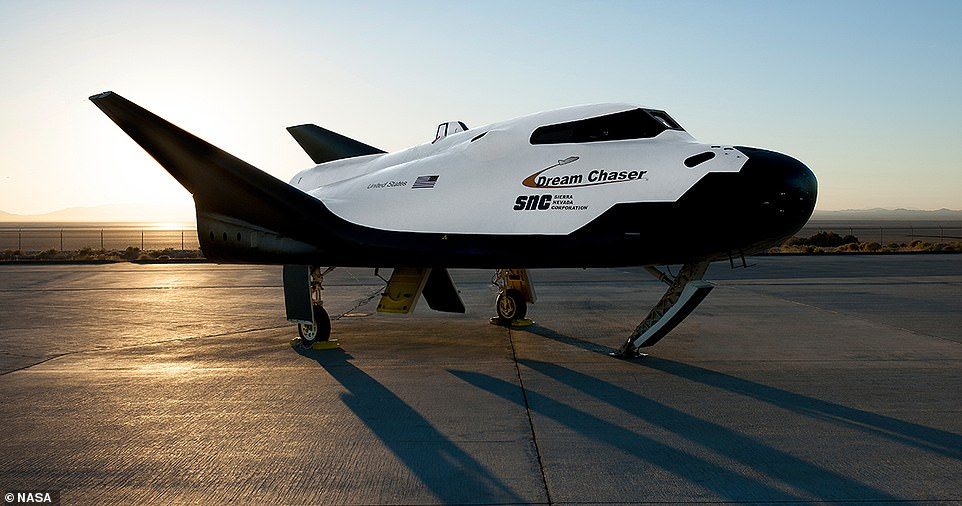
\includegraphics[width=0.9\linewidth, keepaspectratio]{art/dream-chaser-landed.jpg}
	\caption{Dream Chaser on a runway at sunset \cite{misc:dccs-landed}}
	\label{fig:dccs-landed}
\end{figure}
Finally, its communication subsystem is made of several types of antennas, for encrypted telecommunication with ground stations and the \gls{ISS}. Because docking to the space station is also one of the spacecraft's capabilities, a physical communication link is present too. \gls{MDA} has been put in charge of this crucial component's development by \gls{SNC}. 

\section{MDA - Industry partner}
\gls{MDA} is one of the greatest actors in the emerging Canadian space industry. In 2018, it composed nearly one-fifth of the total number of space sector jobs in the country\cite{online:mda-front-page}\cite{misc:canada-space-industry-report}. The Canada-based company, which has offices in Montreal, has already partnered on multiple occasions with the Canadian Space Agency. It's most notable contributions are the design and manufacturing of the Canadarm2 on the \gls{ISS}, as well as the RADARSAT-2 satellite constellation. This thesis was made in partnership with \gls{MDA}, in the context of a 6 months thesis-internship in Montreal during which the present project was scoped, planned and executed. The work was officially supervised by Claudio Discepola, Senior member of the Dream Chaser team. 

\section{Background}\label{sec:intro-background}
With the ever decreasing cost of computing power, functional simulation of components and systems has become an integral part of the testing phase in space design. This approach is thus also taken by \gls{SNC} in the context of Dream Chaser, who requires subcontractors like \gls{MDA} to provide simulators of their respective subsystems alongside the subsystem itself. This is done with the intent of simulating, on multiple fronts, an entire launch or mission, from the reception and handling of telecommands to the behavior of the flight computer mid-mission. 

Once the simulators are all working separately, they are then interfaced together. This results in a compute-intensive platform called the \gls{DCMS}, an important piece in the integration, testing and validation phases of the development. By its virtual nature, the \gls{DCMS} can be ran under different conditions in order to observe the behavior of the spacecraft as a whole in different scenarios. This proves to be  very useful, for example, in the early detection of anomalies or also in the regression testing of software.

Each subcontractor's simulator possesses its own set of requirements, driven by the desired simulation quality and granularity. In that sense, \gls{MDA} is in charge of developing the \gls{BBPSim}, a \gls{SIL} platform for the flight code of the entire communication subsystem, from the antennas to the computing nodes themselves. \gls{BBPSim} acts as some sort of hypervisor, exposing an interface to operating system and hardware utilities to the flight software, itself fundamentally written for an embedded platform. This makes abstraction of the system on which the code is running while keeping all of its functionalities and internal algorithms. As a result, \gls{BBPSim} significantly improves the easiness of interaction with the flight software as well as enabling its testing on a Linux machine in a continuous integration pipeline system like Jenkins.

\section{Purpose}
The purpose of this thesis is to design and develop a custom-fit \textit{snapshotting} technique for \gls{BBPSim}. As said previously, the development of the simulator is driven by the requirements derived from its inclusion in the DCMS. The need for a snapshot feature comes from a pair of them, that state that
\begin{enumerate}
	\item \gls{BBPSim} shall have the capability of saving its state, or "context", to non-volatile memory.
	\item \gls{BBPSim} shall be able to restore itself from a state file in non-volatile memory at initialization.
\end{enumerate} 

This snapshotting feature (often called the \textit{Save \& restore} in the document) will be a considerable addition to the \gls{BBPSim} framework. It will add the possibility to exhaustively represent an on-going simulation at a definite time $t$. It is called a snapshot due to its many similarities with virtual machine software like the open-source VirtualBox. In VirtualBox, it is possible for the user to pause, or to "snapshot" a running instance of a virtual machine, to save it into a relatively large file (called state file) and to restore everything back exactly like it was: running programs, graphics card output and general OS state are all recovered.  

Save \& restore has considerable advantages from a testing point of view. For instance, in the context of Dream Chaser, the flight software enters different states depending on the phase of launch the spacecraft is in. The code doesn't have the same behavior during the launch phase than it has when in the docking phase. However, for the software to change state, some sort of outside stimuli must happen. This external manipulation, albeit automatically executed, can last many minutes for each test. Considering there are hundreds of tests, the time for exhaustive regression testing is of course significant. The snapshot feature completely removes that limitation, because it enables the simulator to be instantly started to a previous state without having to interact with the \gls{FSW}. It is possible to shortcut directly to the docking phase without having to go trough simulating the launch phase. 

Furthermore, another benefit of the feature is that it allows the same hypothetical failures to be replayed over and over again. Since a state file can be restored again and again at will, the interaction between all the different subsystems can be analyzed more in-depth. When in the integration phase, potential inter-system faults can be caught earlier and they are easier to reproduce.  

\section{Thesis Overview TO BE UPDATED}
This thesis will start by giving an general idea of such a \textit{snapshotting} concept in the context of other software projects. There has been many successful attempts to create this mechanism in academic papers and open-source programs, instances from which inspiration has been drawn. Then, the design and implementation of the feature inside \gls{BBPSim} is discussed in details. The general approach in terms of changing the simulator's software to make it saveable is explained. After these crucial steps, the integration of the work in the existing testing pipeline as well as its impact on the testing process at MDA are also covered. 

The rest of this paper is organized as follows. In Section 2, we present background
for and define the problem. In Section 3, we define some terminology and describe
our basic approach. In Section 4, we discuss some of the difficulties of adding faulttolerance to MPI programs. In Sections 5 and 6 we present non-blocking checkpointing
protocols for point-to-point and collective communication, respectively. In Section 7,
we discuss how our system saves the sequential state of each process. In Section 8, we
present performance results of our system. In Section 9 we discuss related work, and in
Section 10 we describe future work. In Section 11, we offer some conclusions.

%\chapter{Conclusion and recommendations}\label{cha:conclusion}

}


% post-content of thesis
\printbibliography[
	heading=bibintoc,
	title={Whole bibliography}
]

\end{document}
